% Драфт секции 3.3 (методы): Максимизация активации в ИНС (MANGO)
% Источник: Pospelov2025 (Neurocomputing), parts/neurotrain/main.tex, строки 226-406
%
% ВНИМАНИЕ: для компиляции блока \begin{algorithm} необходимо добавить в
% Dissertation/userpackages.tex:
%   \usepackage[ruled]{algorithm2e}
%   \RestyleAlgo{ruled}

% ============================================================================
% 3.3.X  Оптимизация латентных представлений стимулов
% ============================================================================

\subsection{Оптимизация латентных представлений стимулов с помощью разложения тензорного поезда}\label{sec:mango_tt}

Как отмечалось выше, задача максимизации активации (МА) в нашей постановке сводится к оптимизации функции чёрного ящика, областью определения которой является латентное пространство генеративной модели размерности $\sim\!10^{2}$. Если дискретизировать ограниченную область этого пространства, результирующий многомерный тензор может обладать низким рангом: как искусственные (по конструкции), так и биологические (в силу физических ограничений) нейронные сети не обладают экспоненциальными ресурсами для кодирования всех точек латентного пространства~\cite{low-rank-in-living-neurons-activity,low-rank-in-living-neurons-activity-2}. При этом предположении эффективными оказываются методы оптимизации, основанные на низкоранговых тензорных разложениях, в частности разложение тензорного поезда (TT-разложение), введённое Оселедцем~\cite{TT-Oseledets}. TT-разложение позволяет представить многомерный тензор в компактном формате, используя полиномиальное (а не экспоненциальное) число параметров относительно размерности тензора. На этой основе построен ряд алгоритмов оптимизации (TTOpt~\cite{TTOpt-paper}, Optima-TT~\cite{Optima-TT-Chertkov}; обзор см.~в~\cite{Cichocki-tensors-for-optimization-1,Cichocki-tensors-for-optimization-2}), в которых целевая функция последовательно аппроксимируется TT-разложением, а кандидат на оптимум находится с использованием структуры тензорного поезда.

Среди методов оптимизации на основе TT наиболее эффективным в нашей задаче оказался метод PROTES (<<Probabilistic Optimization with Tensor Sampling>>)~\cite{PROTES-Chertkov-paper}. Его основная идея напоминает имитацию отжига~\cite{Simulated-annealing-what-is}: в отличие от градиентных методов, застревающих в локальных оптимумах, PROTES обладает вероятностным механизмом выхода из них. Схема метода описана в~\cite{PROTES-Chertkov-paper}.

Для целевой функции $f(\mathbf{x})$ (минимизируемой; максимизация выполняется минимизацией $-f(\mathbf{x})$) вводится монотонное преобразование Ферми--Дирака:
\begin{equation*}
    F[f](x) = \frac{1}{
        \exp \bigl(
            (f(\mathbf{x}) - y_{\text{min}} - E) / T
        \bigr)
        + 1
    },
\end{equation*}
где $y_\text{min}$ --- точный или приближённый минимум $f$, $T>0$ --- параметр <<температуры>>, $E$ --- пороговое значение <<энергии>>. Функция $F$ играет роль, подобную функции распределения: максимум её математического ожидания $\max_\theta \mathbb{E}_{\xi_\theta} F[f](\xi_\theta)$ может быть найден стабильно для семейства случайных величин $\xi_\theta$ с параметрическим распределением $p_\theta(\mathbf{x})$. С помощью трюка REINFORCE~\cite{REINFORCE-trick} градиент этого ожидания оценивается методом Монте-Карло:
\begin{equation}
    \nabla_\theta\mathbb{E}_{\xi_\theta}F[f](\xi_\theta)\approx \frac{1}{M}\sum_{i=1}^M
    F[f](\mathbf{x}_i)\nabla_\theta \log p_\theta(\mathbf{x}_i),
    \label{expectation-gradient}
\end{equation}
где $\{\mathbf{x}_i\}_{i=1}^{M}$ --- независимые реализации $\xi_\theta$. При <<низкой температуре>> (малых $T$) лишь несколько членов вносят вклад в сумму~(\ref{expectation-gradient}) --- а именно те $\mathbf{x}_i$, для которых $f(\mathbf{x}_i)-y_\text{min}<E$ (<<частицы низкой энергии>>), --- что фактически сводит процедуру к отбору нескольких лучших кандидатов из выборки. Если $p_\theta$ допускает низкоранговое TT-представление, выборка и отбор лучших значений выполняются быстро и эффективно.


% ============================================================================
% 3.3.X  Обучение модельных нейронных сетей и генеративных моделей
% ============================================================================

\subsection{Обучение модельных нейронных сетей и генеративных моделей}\label{sec:mango_models}

\textbf{Импульсная нейронная сеть.}
В качестве целевой модели для экспериментов по МА использовалась импульсная нейронная сеть на основе архитектуры ResNet18~\cite{ResNet-paper}, реализованная с помощью библиотеки SpikingJelly~\cite{SpikingJelly-paper}. Сеть содержала нейроны с утечкой и накоплением (LIF) с константой затухания мембранного потенциала $\beta = 0{,}9$ (см. описание модели LIF в разделе~\ref{sec:lit_ann_repr}). Обучение проводилось методом суррогатного градиента, без использования локальных правил обучения. Время дискретизировалось на $T = 50$ отсчётов; активность отдельного нейрона определялась числом генерируемых им импульсов за время экспозиции стимула. Обученная сеть достигла точности классификации 86\% на наборе данных CIFAR-10~\cite{CIFAR10-dataset-reference}. Активность усреднялась по всем каналам признаков каждого слоя и нормализовалась к диапазону $[0, 1]$.

\textbf{Генеративная модель.}
Для отображения латентного пространства стимулов в пространство изображений были протестированы две генеративные архитектуры: спектрально-нормализованная генеративно-состязательная сеть (SN-GAN)~\cite{SN-GAN-paper} и векторно-квантованный вариационный автокодировщик (VQ-VAE)~\cite{VQ-VAE-Van-Den-Oord}. SN-GAN продемонстрировала лучшее качество генерации стимулов в нашей постановке (сравнение производительности обеих моделей приведено в приложении). В итоговой конфигурации использовалась SN-GAN с латентным пространством размерности 128, где каждое измерение было дискретизировано на 64 части.


% ============================================================================
% 3.3.X  Алгоритм построения наиболее активирующих изображений
% ============================================================================

\subsection{Алгоритм построения наиболее активирующих изображений}\label{sec:mango_algorithm}

Для систематического вычисления наиболее активирующих изображений (MEI) был разработан программный фреймворк MANGO (<<Максимизация нейронной активации посредством безградиентной оптимизации>>). Фреймворк объединяет генеративную модель, целевую нейронную сеть и оптимизатор в единый конвейер, схема которого показана на рис.~\ref{nt:MANGO-framework}.

\begin{figure}[ht]
\centering
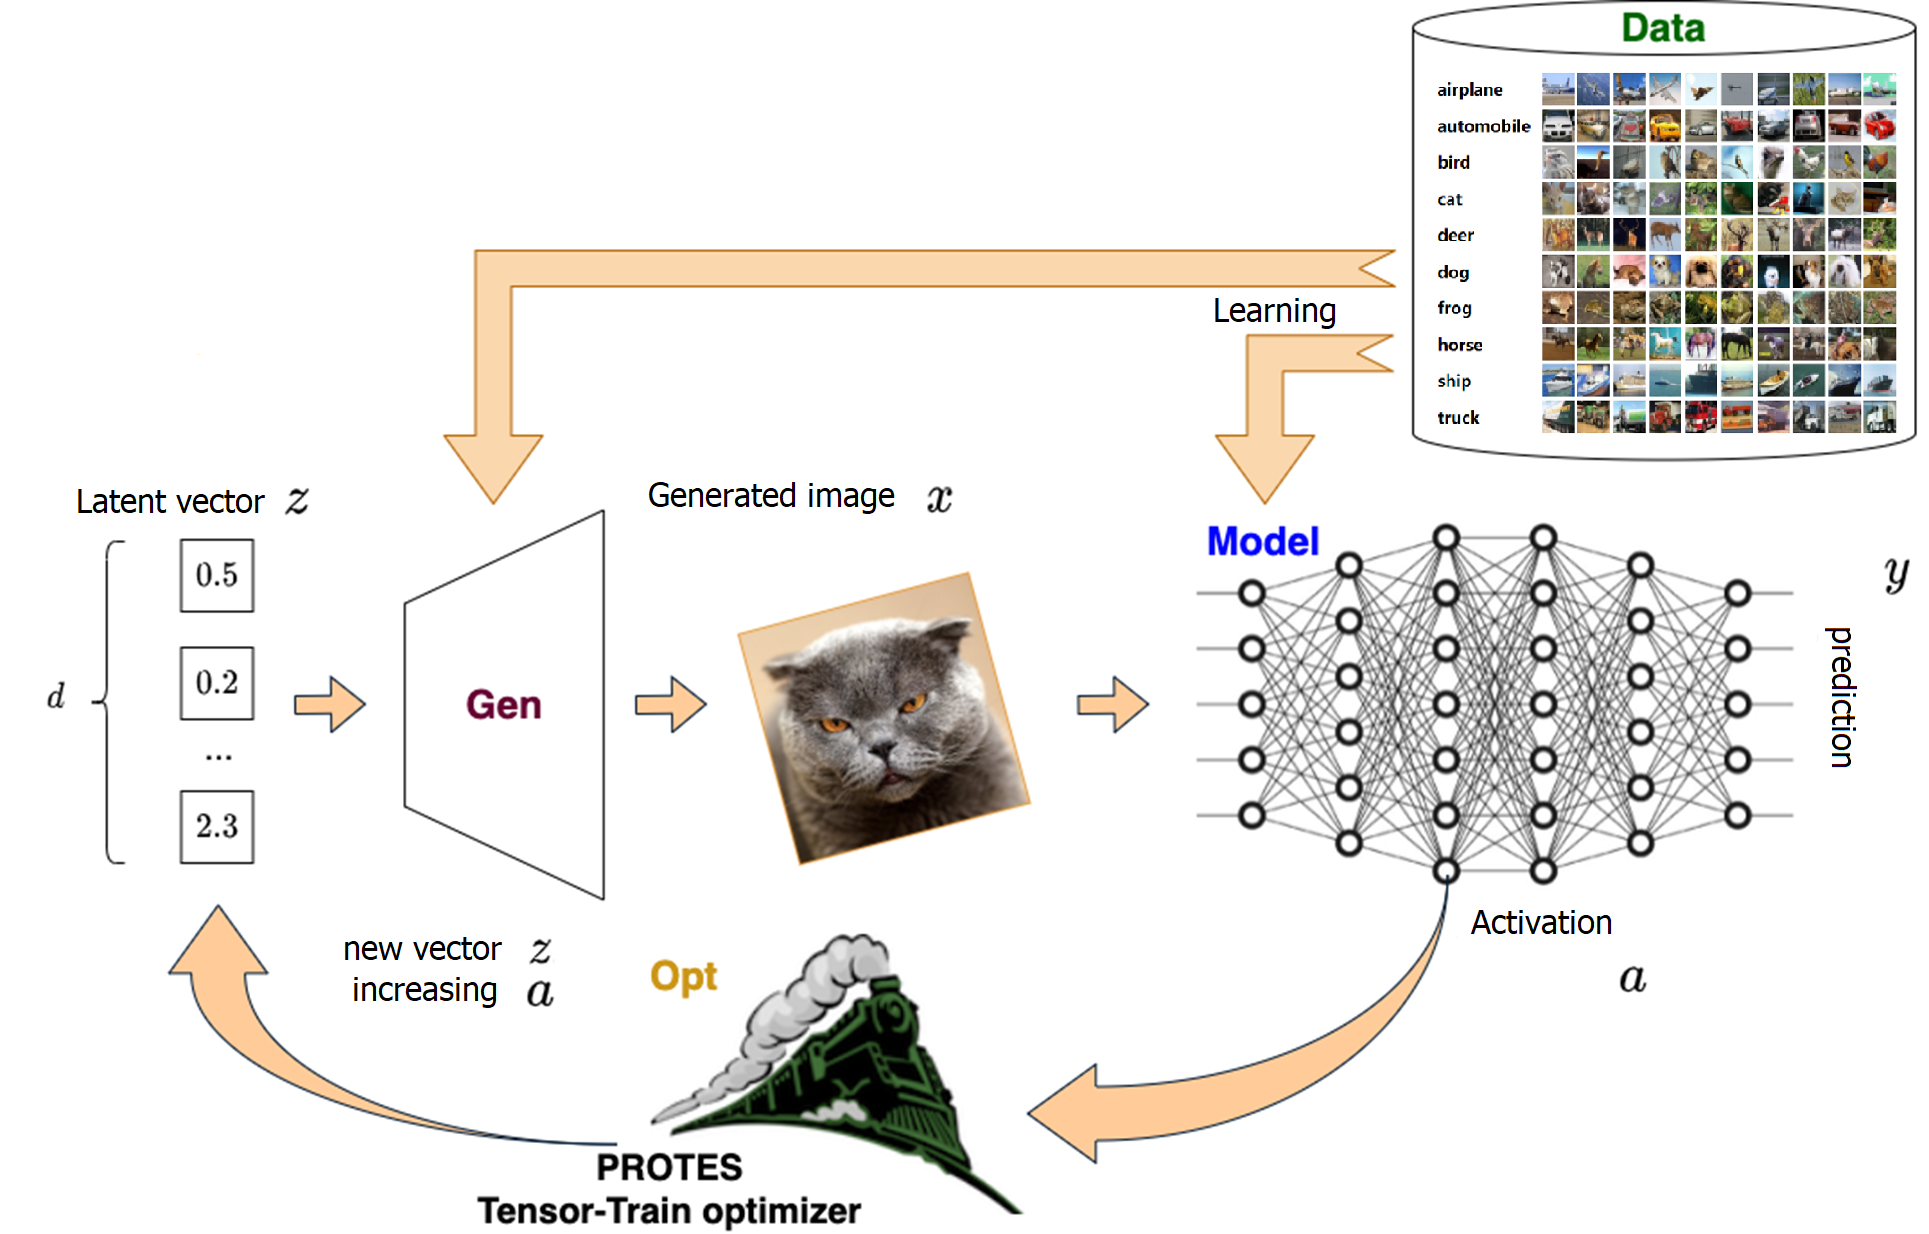
\includegraphics[width=0.95\textwidth]{images/neurotrain/MANGO.png}
\caption{Схема фреймворка MANGO.}
\label{nt:MANGO-framework}
\end{figure} В рамках MANGO выбранный набор данных используется для обучения классификатора и генератора. После обучения генератор создаёт латентные представления стимулов, которые преобразуются в изображения и предъявляются классификатору. Активация интересующего нейрона измеряется и передаётся оптимизатору, который генерирует улучшенный латентный вектор, максимизирующий ответ данного нейрона. Процесс повторяется до сходимости или исчерпания бюджета запросов.

Алгоритм~\ref{alg:mango} описывает процедуру построения MEI на основе метода PROTES.

\begin{algorithm}[H]
\caption{Построение MEI с использованием PROTES}\label{alg:mango}
\footnotesize
\KwData{функция, которая вычисляет активацию целевого нейрона $a = f(x)$ для любого входного изображения $x \in \mathrm{R}^{d_{inp}}$, имеющего $d_{inp}$ пикселей;
    генеративная модель $x = g(z)$, которая создает искусственный вход (изображение) $x$ для предоставленного латентного вектора $z \in \mathrm{R}^{d}$, где $d$ -- размерность латентного пространства;
    максимальное количество запросов $m$ (т.е. вычислительный бюджет).}
\KwResult{
    входное изображение $x^{(opt)}$, которое максимизирует активацию.
}

\SetKwFunction{FMain}{loss}
\SetKwProg{Fn}{Function}{:}{}
\Fn{\FMain{$z$}}{
    Генерировать искусственный вход (изображение):
    $
    x = g(z)
    $

    Вычислить активацию нейрона:
    $
    a = f(x)
    $

    \KwRet $a$
}

Оптимизировать до исчерпания бюджета:
$
z^{(opt)} =
    \mathrm{protes}(\mathrm{loss}, \mathrm{budget}=m)
$

Оптимизатор последовательно генерирует кандидатов для оптимума, выполняет соответствующие запросы к целевой функции и обновляет внутренний тензор ожидания для оптимума на основе возвращённых значений. См. алгоритм 1 с деталями метода оптимизации PROTES в оригинальной работе~\cite{PROTES-Chertkov-paper}.

Генерировать искусственный вход (изображение):
$
x^{(opt)} = g(z^{(opt)})
$

\Return{$x^{(opt)}$}

\end{algorithm}

В экспериментах проводилось сравнение следующих методов оптимизации:
\begin{enumerate}
    \itemsep0em
    \item Случайный поиск (базовый метод).
    \item Portfolio из пакета Nevergrad~\cite{Nevergrad} (базовый метод) --- объединение стратегии эволюции с адаптацией ковариационной матрицы (CMA-ES), дифференциальной эволюции (DE) и SCR-Hammersley.
    \item PROTES~\cite{PROTES-Chertkov-paper} с размером выборки $K=10$ и числом лучших кандидатов $k_\mathrm{top}=1$.
    \item TT-s --- PROTES с $K=5$, $k_\mathrm{top}=1$ и квантованием тензорных мод (преобразование каждого измерения в набор измерений с меньшими модами).
    \item TT-b --- PROTES с $K=25$, $k_\mathrm{top}=5$ и квантованием мод.
\end{enumerate}
Для всех вариантов PROTES гиперпараметр тензорного ранга был установлен $r = 5$: каждый <<вагон>> аппроксимации тензорного поезда представлял собой тензор ранга~5. Эксперименты с различными значениями $r$ в близлежащем диапазоне давали сопоставимые результаты.

Код MANGO доступен на GitHub\footnote{\url{https://github.com/iabs-neuro/mango}}, включая скрипты обучения и анализа.
